\documentclass[a4paper,11pt]{article}
\usepackage{a4wide}
\usepackage{fullpage}
\usepackage[utf8x]{inputenc}

%\usepackage[light,math]{anttor}
\usepackage[T1]{fontenc}

\usepackage[slovene]{babel}
%\selectlanguage{slovene}
\usepackage[toc,page]{appendix}
\usepackage[pdftex]{graphicx} 

\usepackage{lmodern}
\usepackage{amsmath}
\usepackage{amssymb}
\usepackage{amsthm}
\usepackage{amsfonts}
\usepackage{mathtools}
\usepackage{enumitem}
\usepackage{amsfonts}
\usepackage{amsmath}
\usepackage{setspace}
\usepackage{relsize}
\usepackage{color}
\definecolor{light-gray}{gray}{0.95}
\usepackage{listings} 
\usepackage{hyperref}
\renewcommand{\baselinestretch}{1.2} 
\renewcommand{\appendixpagename}{Priloge}

\lstset{ 
language=Matlab,
basicstyle=\footnotesize,
basicstyle=\ttfamily\footnotesize\setstretch{1},
backgroundcolor=\color{light-gray},
}

%\usepackage{algorithm}
%\usepackage[noend]{algpseudocode}

\theoremstyle{definition} 
\newtheorem*{definicija}{Definicija}
\newtheorem*{trditev}{Trditev}


\theoremstyle{plain} 
\newtheorem*{izrek}{Izrek}
\newtheorem*{posledica}{Posledica}
\newtheorem*{zgled}{Zgled}
\newtheorem{primer}{Primer}

\title{Krožnica in ostale stožnice \\
v racionalni B\'ezierjevi obliki
}
\author{Sara Bizjak in Urša Blažič}
\date{\today}

%%%%%%%%%%%%%%%%%%%%%%%%%%%%%%%%%%%%%%%%%%%%%%%%%%%%%%%%%%%%%%%%%%%%%%%%%%%%%%%%%%%%%%

\begin{document}

\maketitle

\section{Uvod}
V seminarski nalogi so predstavljene krožnice in ostale stožnice v racionalni B\'ezierjevi obliki. Med tem ko so stožnice na splošno omenjene le v grobem, pa se v krožnice bolj poglobimo in jih podamo natančneje.

Najprej se na splošno seznanimo z racionalnimi B\'ezierjevimi krivuljami in jih poslošimo na stožnice. Iz stožnic preidemo na krožnico in si jo natančeneje pogledamo. Ugotovimo, kako lahko dobimo sklenjeno krožnico z racionalno krivuljo čim nižje stopnje in jo konstruiramo.


%%%%%%%%%%%%%%%%%%%%%%%%%%%%%%%%%%%%%%%%%%%%%%%%%%%%%%%%%%%%%%%%%%%%%%%%%%%%%%%%%%%%%%

\section{Racionalne B\'ezierjeve krivulje}

Racionalna B\'ezierjeva krivulja stopnje $n$ v $\mathbb{R}^d$ je projekcija polinomske B\'ezierjeve krivulje stopnje $n$ v $\mathbb{R}^{d+1}$ na hiperravnino $w=1$, kjer točko v  $\mathbb{R}^{d+1}$  označimo z
$$(\boldsymbol{x},w)=(x_1,x_2,\dots,x_d,w).$$
Projekcija je definirana kot
$$(\boldsymbol{x},w)\mapsto (\frac{1}{w}\boldsymbol{x},1).$$
Točke oblike $\lambda(\boldsymbol{x}, w)$ za $\lambda\neq 0$ se preslikajo v isto točko na projektivni ravnini, točke z
$w = 0$ pa predstavljajo točke v neskončnosti.

\begin{definicija}
\emph{Racionalna B\'ezierjeva krivulja} stopnje $n$ je podana s parametrizacijo $\boldsymbol{r}:[0,1]\rightarrow \mathbb{R}^d$, določeno s predpisom
$$\boldsymbol{r}(t)=\frac{\mathlarger{\sum}_{i=0}^n w_i\boldsymbol{b}_iB_i^n(t)}{\mathlarger{\sum}_{i=0}^n w_iB_i^n(t)},$$
kjer so $\boldsymbol{b}_i$ kontrolne točke krivulje, $w_i\in\mathbb{R}^d$ uteži, $B_i^n$ pa $i$-ti Bernsteinov bazni polinom stopnje~$n$.
\end{definicija}
 
Krivuljo lahko brez škode za splošnost reparametriziramo tako, da sta $w_0$ in $w_n$ enaka $1$. Taki obliki pravimo \emph{standardna oblika} racionalne B\'ezierjeve krivulje.
Ostale uteži so prosti parametri, ki vplivajo na obliko krivulje -- s povečanjem enega izmed $w_i$ se krivulja približa ustreznemu $\boldsymbol{b}_i$. Racionalne B\'ezierjeve krivulje s pozitivnimi utežmi imajo podobne lastnosti kot polinomske. \\
Povzeto po \cite{knez}.

%%%%%%%%%%%%%%%%%%%%%%%%%%%%%%%%%%%%%%%%%%%%%%%%%%%%%%%%%%%%%%%%%%%%%%%%%%%%%%%%%%%%%%

\section{Stožnice v racionalni B\'ezierjevi obliki}
Stožnice bomo zapisali s pomočjo krivulje stopnje $2$, zato bo kontrolni poligon sestavljen iz treh kontrolni točk. Ker lahko izberemo uteži v standardni obliki, velja: 
$$w_0=w_2=1 $$
in
$$ w_1=w,$$
kjer je $w_1$ prosta utež.
\\
Stožnice lahko zapišemo v racionalni B\'ezierjevi obliki kot 
$$\boldsymbol{r}(t)=\frac{\boldsymbol{b}_0\cdot B_0^2+w\cdot\boldsymbol{b}_1\cdot B_1^2+\boldsymbol{b}_2\cdot B_2^2}{ B_0^2+w\cdot B_1^2+ B_2^2},\,\,\, t\in[0,1],$$
kjer so $\boldsymbol{b}_0, \boldsymbol{b}_1, \boldsymbol{b}_2 \in \mathbb{R}^2$ kontrolne točke krivulje, $w$ utež, vezana na kontrolno točko $\boldsymbol{b}_1$, $B_i^2,\,i=~0,1,2,$ pa Bernsteinovi bazni polinomi:

\begin{align*}
B_0^2(t) &= (1-t)^2 \\
B_1^2(t) &= 2t\cdot(1-t) \\
B_2^2(t) &= t^2 \\
\end{align*}

Ker uteži, kot že omenjeno, izbiramo v standardni obliki, je srednja utež $w_1$ prosti parameter, ki vpliva na obliko krivulje. Če utež $w_1$ povečujemo, se krivulja približuje kontrolni točki $b_1$, kot je prikazano na sliki \ref{slika:w1}.

\begin{figure}[ht!]
    \centering
    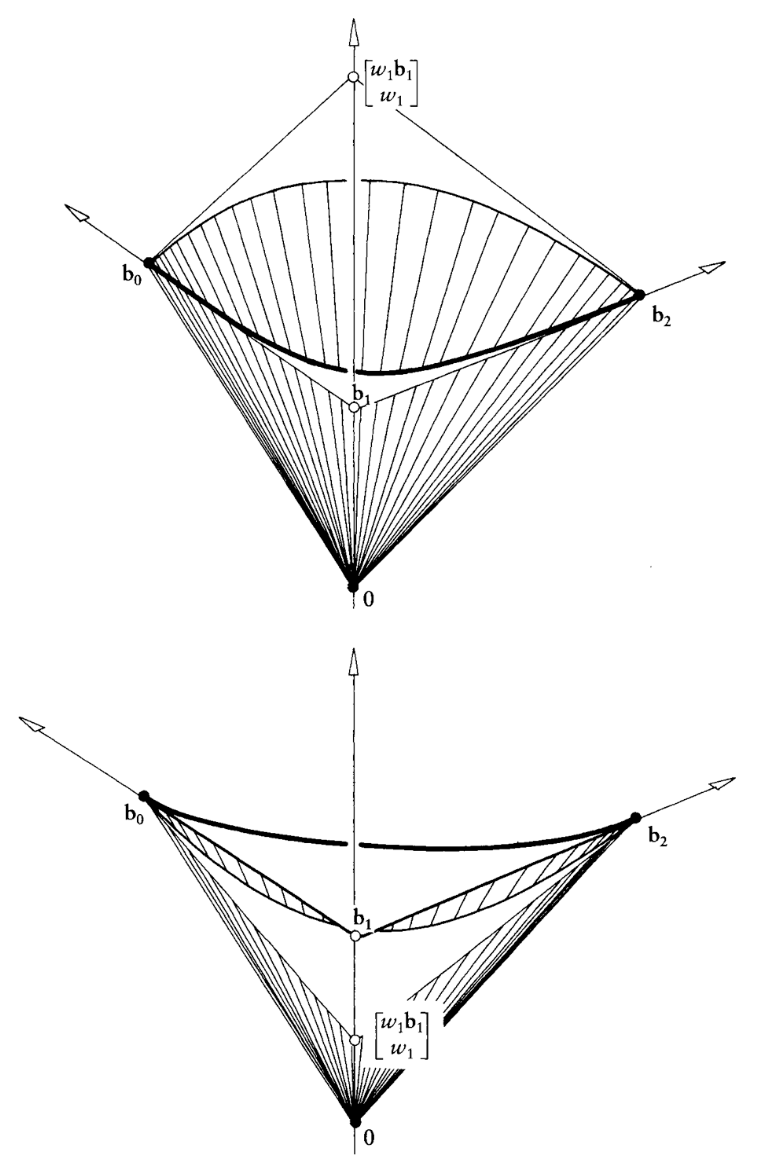
\includegraphics[width=70mm]{vecanje_w1.png}
    \caption{Krivulji na obeh slikah sta v standardni obliki, torej velja $w_0 = w_2 = 1$. Sliki prikazujeta večanje uteži $w_1$, to je približevanje krivulje h kontrolni točki $b_1$. Slika je povzeta po \cite{farin}.}
    \label{slika:w1}
\end{figure}

\newpage
Spreminjanje uteži $w_1$ in vpliv na obliko krivulje lahko klasificiramo v tri skupine. Če je $w_1 < 1$, ima krivulja obliko elipse, če je $w_1 = 1$, je krivulja parabola, za $w_1 > 1$ pa dobimo hiperbolo. Omenjeni trije tipi krivulj so prikazani na sliki \ref{slika:klasifikacija}.

\begin{figure}[ht!]
    \centering
    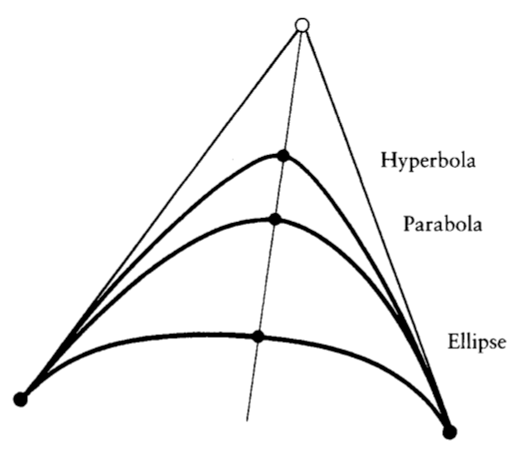
\includegraphics[width=70mm]{tri_oblike.png}
    \caption{Klasifikacije krivulje glede na spreminjanje srednje uteži $w_1$ pri predpostavki, da velja $w_0 = w_2 = 1$. Slika je povzeta po \cite{farin}.}
    \label{slika:klasifikacija}
\end{figure}
\noindent
Ena izmed najpomembnejših stožnic je krog, zato mu v nadaljevanju posvetimo več pozornosti.


%%%%%%%%%%%%%%%%%%%%%%%%%%%%%%%%%%%%%%%%%%%%%%%%%%%%%%%%%%%%%%%%%%%%%%%%%%%%%%%%%%%%%%

\section{Krožnica v racionalni B\'ezierjevi obliki}

\subsection{Motivacija}

Naj kvadratična krivulja z utežjo $w_1 < 1$ opiše krožni lok. Ker je krog simetričen, mora kontrolni poligon tvoriti pravilni $n-$kotnik.
Če poznamo kot v v liku, označimo ga z $\alpha$, lahko določimo utež $w_1$ kot $w_1 = \text{cos} \alpha$.
Celoten krog lahko tedaj predstavimo kot zlepek večih takih krožnih lokov. 

\begin{figure}[ht!]
    \centering
    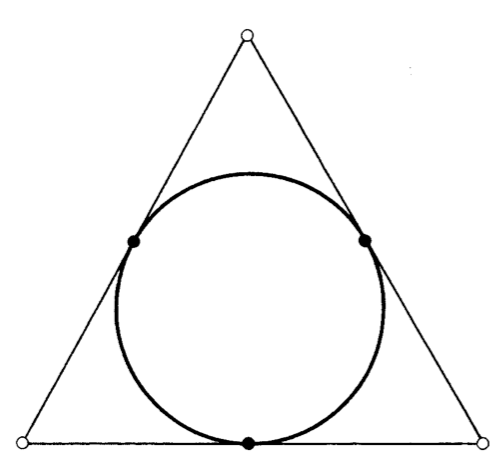
\includegraphics[width=60mm]{krog_po_delih.png}
    \caption{Celoten krog lahko sestavimo iz treh racionalnih kvadratičnih B\'ezierjevih krivulj. Slika je povzeta po \cite{farin}.}
    \label{slika:krogpodelih}
\end{figure}
\noindent
Na sliki \ref{slika:krogpodelih} je prikazan primer, ko je kontrolni poligon enakostranični trikotnik, to pomeni, da je kot $\alpha$ velik 60 stopinj. Velja torej elja $w_1 = \frac{1}{2}$. V tem primeru je krog sestavljen iz treh enakih krožnih lokov.
\\

Namesto, da krožnico opisujemo z zlepkom krivulj, bi jo želeli opisati z eno samo racionalno krivuljo čim nižje stopnje.
\\
Nadalje si najprej oglejmo formalno definicijo krožnice v racionalni B\'ezierjevi obliki in problem iskanja racionalne krivulje čim nižje stopnje, ki opiše krožnico, reducirajmo na lažjega.

\subsection{Formulacija krožnice v racionalni B\'ezierjevi obliki}
Krožnico lahko opišemo kot racionalno B\'ezierjevo krivuljo $\boldsymbol{C}(t)=(X(t),Y(t))$ s pomočjo projekcije krivulje $\boldsymbol{\tilde{C}}(t)=(\tilde{X}(t), \tilde{Y(t)}, W(t))$ na ravnino $w=1$. 
Enačbo krožnice v $\mathbb{R}^2$ lahko zapišemo kot
$$X(t)^2+Y(t)^2=1.$$
Koordinate točk zamenjamo s koordinatami prostora $\mathbb{R}^3$, ki smo jih dobili s projekcijo na ravnino $w=1$.
$$\left(\frac{\tilde{X}(t)}{W(t)}\right)^2+\left(\frac{\tilde{Y}(t)}{W(t)}\right)^2=1$$
$$\tilde{X}(t)^2+\tilde{Y}(t)^2-W(t)^2=0$$
Zadnja enačba predstavlja enačbo stožca. Vidimo, da racionalna krivulja $\boldsymbol{C}(t)$ eksaktno opiše krožnico kot projekcijo krivulje $\boldsymbol{\tilde{C}}(t)$ (ki leži na stožcu) na ravnino $w = 1$.

\begin{figure}[ht!]
    \begin{minipage}{0.5\textwidth}
        \centering
        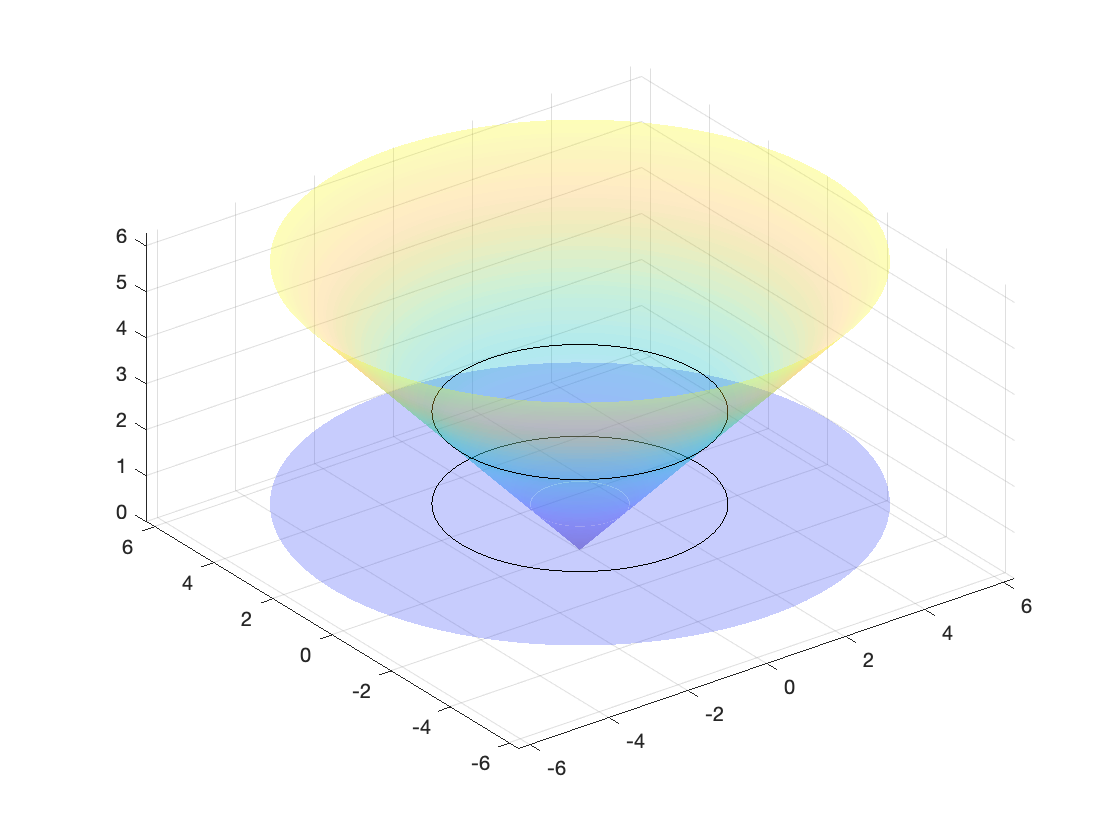
\includegraphics[width=80mm]{stozec.png}
    \end{minipage}\hfill
    \begin{minipage}{0.5\textwidth}
        \centering
        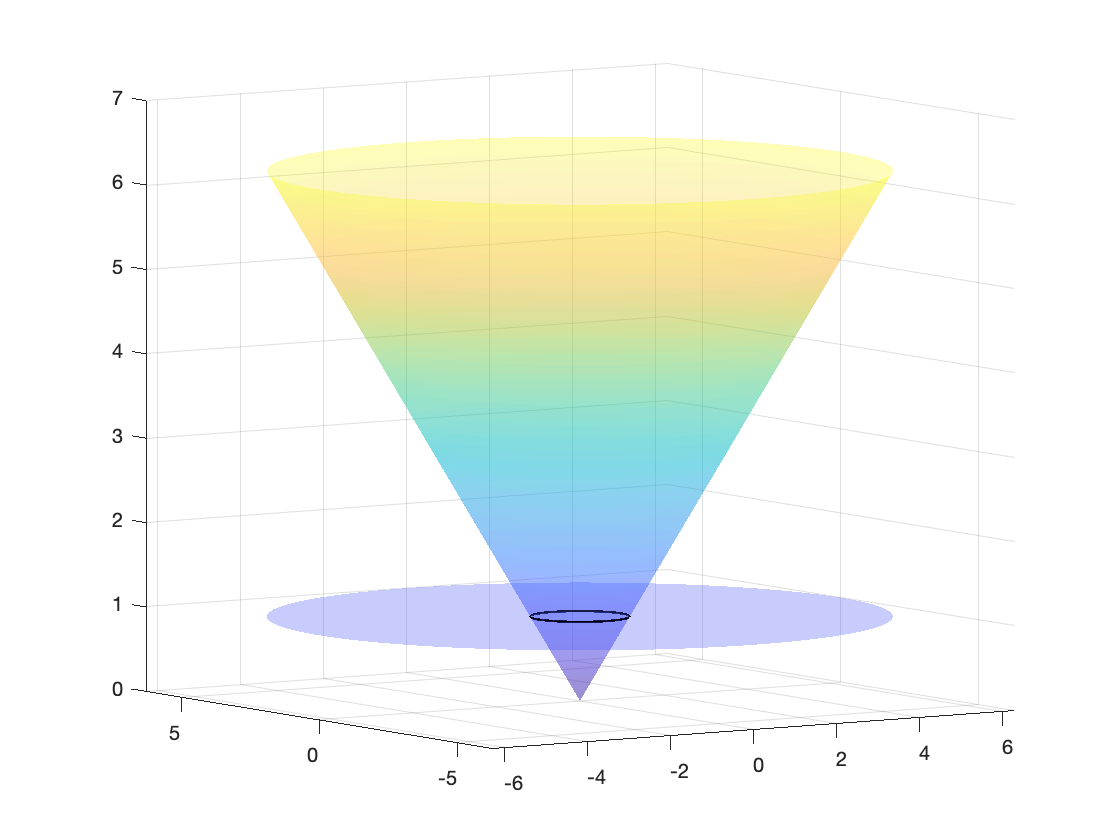
\includegraphics[width=80mm]{stozec_1.png}
    \end{minipage}\hfill
    \caption{Krožnico lahko dobimo kot projekcijo krivulje, ki leži na stožcu, na ravnino $w = 1$.}
\end{figure}
\noindent
Iskanje racionalne krivulje čim nižje stopnje, ki eksaktno opiše celotno krožnico, lahko torej prevedemo na problem iskanja krivulje, ki leži na stožcu. 
\\
V naslednjih podpoglavjih bomo preučili B\'ezierjeve krivulje, ki tvorijo celoten krog. 
Še posebej nas bodo zanimale take krivulje, ki imajo same pozitivne uteži, saj bo take krivulje tudi lažje implementirati.
\\
Začeli bomo s kvadratično B\'ezierjevo krivuljo in nadaljevali s krivuljami z naraščajočim polinomskim redom.

%%%%%%%%%%%%%%%%%%%%%%%%%%%%%%%%%%%%%%%%%%

\subsection{ Kvadratična krivulja}\label{kvadraticna}
Pokazali bomo, da racionalna kvadratična krivulja ne more opisati celotne krožnice. Do tega nas privede enostaven razmislek. 
Vse neracionalne kvadratične B\'ezierjeve krivulje so parabole, vse parabole pa dobimo kot presek stožca z ravnino, ki je vzporedna eni od nosilk stožca. 
\begin{figure}[ht!]
    \begin{minipage}{0.5\textwidth}
        \centering
        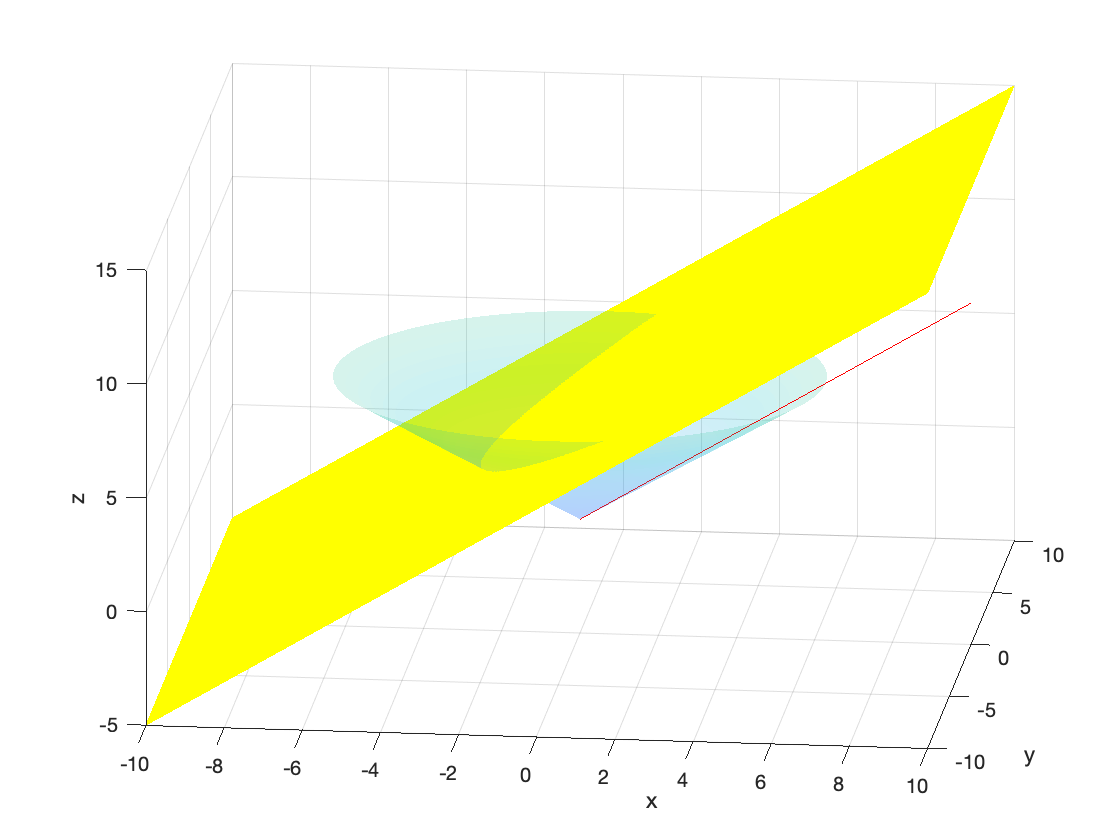
\includegraphics[width=80mm]{stozec_presek_1.png}
    \end{minipage}\hfill
    \begin{minipage}{0.5\textwidth}
        \centering
        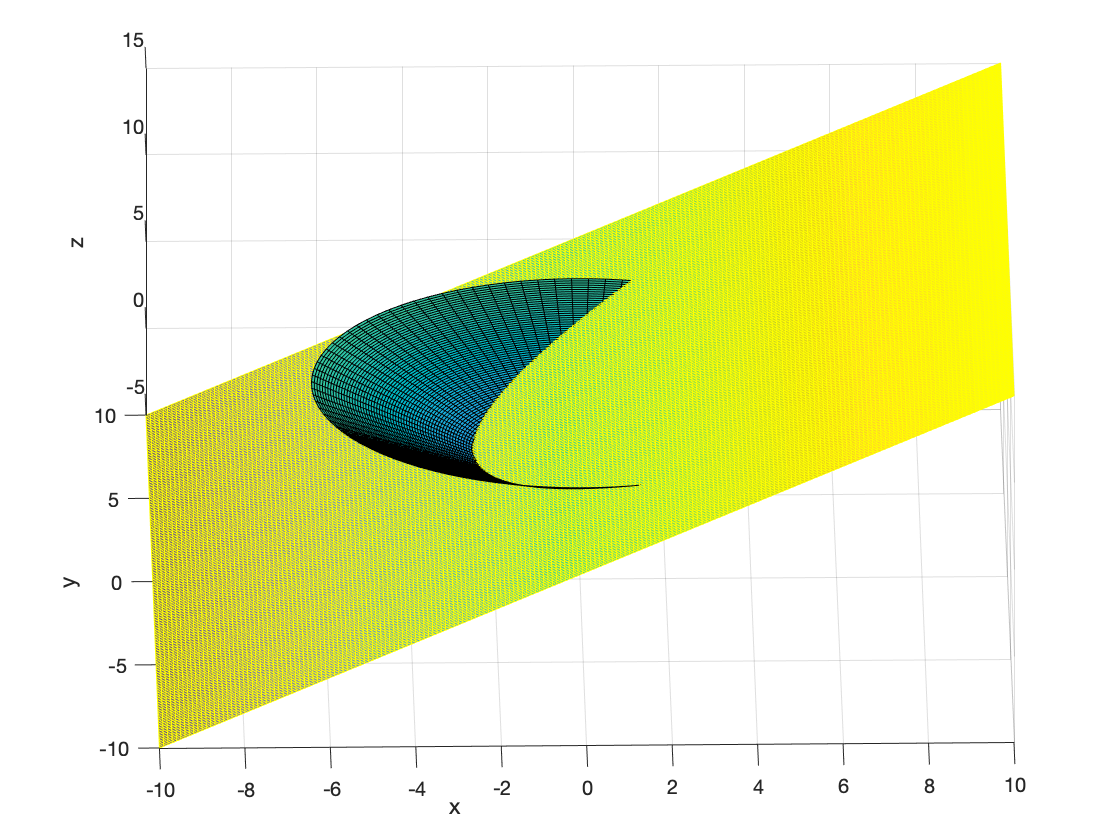
\includegraphics[width=80mm]{stozec_presek_2.png}
    \end{minipage}\hfill
    \caption{Presek stožca z ravnino, ki je vzporedna njegovi nosilki. Na sliki je ravnina obarvana z rumeno barvo, nosilka pa z rdečo.}
\end{figure}

\noindent
Ko ravnino, s katero presekamo stožec, premikamo proti nosilki stožca, opazimo, da bo krožni lok v projekciji na ravnino opisal vedno večji kot, torej smo vedno bližje polnemu krogu. 
Ko pa se ravnina, s katero stožec sekamo, in nosilka stožca ujameta, je njun presek premica, ki se v projekciji slika v eno točko. 
Krožnice zato ne moremo zapisati s kvadratično racionalno krivuljo. 

\noindent
Opazimo pa, da lahko s parabolo zapišemo krožne loke, ki jih opišemo z naslednjim kontrolnim poligonom:
\begin{align*}
\boldsymbol{\tilde{b}}_0 &= (\cos{\theta}, -\sin{\theta}, 1)\\
\boldsymbol{\tilde{b}}_1 &= (1, 0, \cos{\theta})\\
\boldsymbol{\tilde{b}}_2 &= (\cos \theta, \sin\theta, 1),
\end{align*}
kjer je $\theta$ polovični kot krožnega loka. 
% Če izberemo samo pozitivne uteži ($\cos{\theta}>0$), je $C(t)$ manj kot $180^{\circ}$, če pa je srednja utež enaka $0$ ($\cos{\theta}=0$), je $C(t)$ točno $180^{\circ}$. ??
% Za prvo in zadnjo točko si izberemo točki, ki ležita na krožnici, srednjo točko pa zaradi simetrije izberemo na polovičnem kotu med njima. Pri tem izberemo take uteži, da zadoščajo enačbi stožca. 

%%%%%%%%%%%%%%%%%%%%%%%%%%%%%%%%%%%%%%%%%%

\subsection{Kubična krivulja}
Pokazali bomo, da tudi racionalna kubična krivulja ne more opisati celotne krožnice. \\
Denimo, da jo lahko, in da je krivulja $\boldsymbol{\tilde{C}}(t)$, ko jo preslikamo na ravnino $w = 1$, torej $\boldsymbol{C}(t)$, krožnica.
Za kontrolni poligon izberemo štiri kontrolne točke, označimo jih $\boldsymbol{b}_0, \boldsymbol{b}_1, \boldsymbol{b}_2, \boldsymbol{b}_3$. Ker gre krivulja skozi prvo in zadnjo kontrolno točko, ju izberemo na stožcu.
Vemo, da so racionalne kubične krivulje sklenjene, zato se bosta ti dve kontrolni točki ob projekciji na ravnino $w = 1$ preslikali v isto točko. 
Zato lahko za prvo in zadnjo kontrolno točko $\boldsymbol{b}_0$ in $\boldsymbol{b}_3$ izberemo kar isto točko, ki že leži na ravnini $w = 1$. 
Ker krivulja $\boldsymbol{\tilde{C}}(t)$ leži na stožcu, mora tangetna na krivuljo v točki $\boldsymbol{b}_0$ (in hkrati tudi $\boldsymbol{b}_3$) ležati na tangetni ravnini stožca v tej isti točki.
Iz tega sledi, da tudi kontrolni točki $\boldsymbol{b}_1$ in $\boldsymbol{b}_2$ ležita na tangetni ravnini. Vemo, da je presek tangetne ravnine s stožcem premica, torej je krivulja $\boldsymbol{C}(t)$ točka.
Tako pridemo do zaključka, da tudi kubične krivulje ne morejo opisati celotne krožnice.
\begin{figure}[ht!]
    \begin{minipage}{0.5\textwidth}
        \centering
        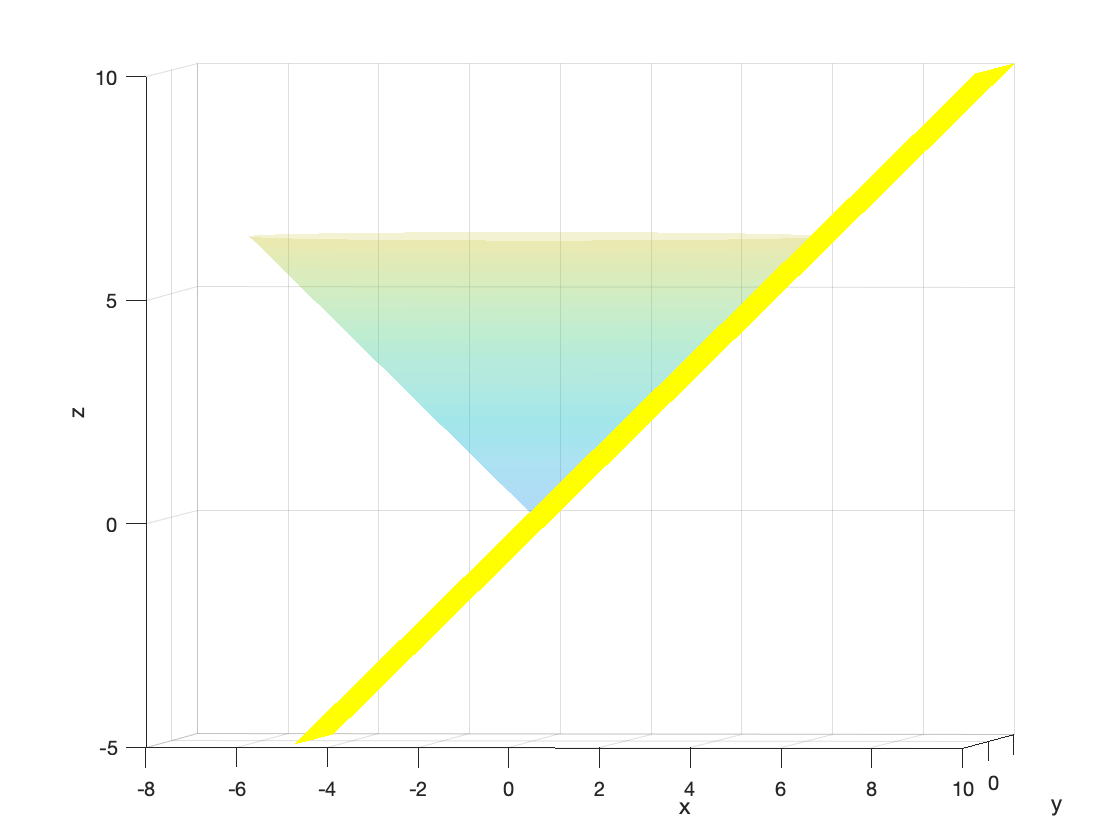
\includegraphics[width=80mm]{stozec_tang_1.png}
    \end{minipage}\hfill
    \begin{minipage}{0.5\textwidth}
        \centering
        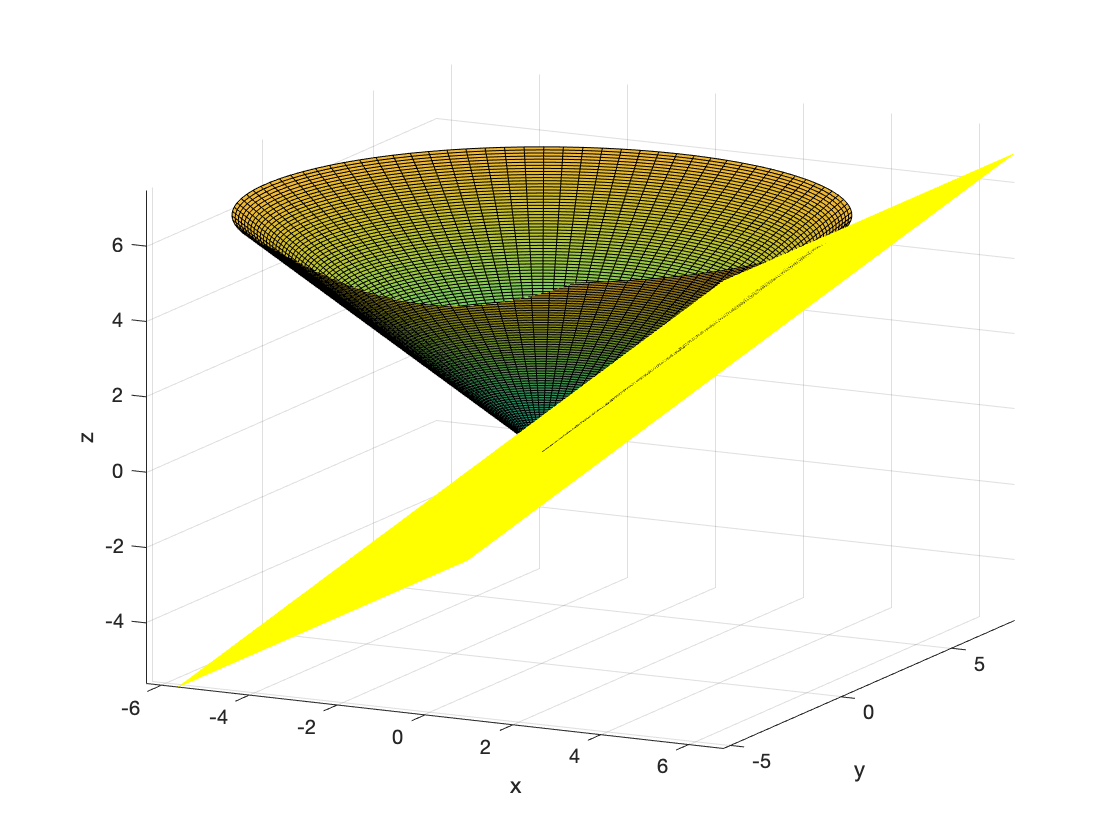
\includegraphics[width=80mm]{stozec_tang_2.png}
    \end{minipage}\hfill
    \caption{Presek stožca s tangentno ravnino. Presek je premica, ki je enaka eni od nosilk stožca.}
\end{figure}

%%%%%%%%%%%%%%%%%%%%%%%%%%%%%%%%%%%%%%%%%%

\subsection{Krivulja 4.~stopnje}
Da bomo dobili vse krivulje, v enačbo za stožec $\tilde{X}(t)^2+\tilde{Y}(t)^2-W(t)^2=0$ vstavimo 
\begin{align*}
\tilde{X}(t) &= \tilde{x}_0\cdot B_0^4(t)+\tilde{x}_1\cdot B_1^4(t)+ \tilde{x}_2\cdot B_2^4(t) + \tilde{x}_3\cdot B_3^4(t) +\tilde{x}_4\cdot B_4^4(t)   \\
\tilde{Y}(t) &=\tilde{y}_0\cdot B_0^4(t)+\tilde{y}_1\cdot B_1^4(t)+\tilde{y}_2\cdot B_2^4(t) + \tilde{y}_3\cdot B_3^4(t) + \tilde{y}_4\cdot B_4^4(t)   
\end{align*}
V enačbi sta $\tilde{X}(t)$ in $\tilde{Y}(t)$ kvadrirana, zato bomo morali med seboj množiti Bernsteinove bazne polinome. Izpeljemo lahko, da velja
$$B_i^n(t)\cdot B_j^m(t)=\frac{\binom{n}{i} \cdot \binom{m}{j}}{\binom{n+m}{i+j}}B_{i+j}^{n+m}(t).$$
Ker smo med seboj množili Bernsteinove bazne polinome stopnje 4, dobimo Bernsteinove bazne polinome stopnje 8. Ker so baza prostora, bo enakost veljala, ko bo seštevek koeficientov pred $i$-tim baznim polinomom enak 0. Iz tega dobimo devet enačb.
Brez škode za splošnost vzamemo $\boldsymbol{\tilde{b}}_0 =\boldsymbol{\tilde{b}}_4 = (1,0,1)$. Ker $\boldsymbol{\tilde{b}}_1$ in $\boldsymbol{\tilde{b}}_3$ ležita v tangentni ravnini $\boldsymbol{\tilde{b}}_0$, velja $\tilde{x}_1=w_1$ in $\tilde{x}_3=w_3$ (saj imamo ravnino $x=w$). Devet enačb se nam tako reducira v pet enačb:
\begin{align*}
\tilde{y}_3 &=- \tilde{y}_1 \\
\tilde{x}_3 &= - \tilde{x}_1 \\
3\tilde{x}_2 + 4\tilde{y}_1^2 - 3w_2 &= 0 \\
\tilde{x}_1\tilde{x}_2 + \tilde{y}_1\tilde{y}_2  - \tilde{x}_1w_2 &= 0 \\
9\tilde{x}_2^2 - 8\tilde{y}_1^2 + 9\tilde{y}_2^2 - 9w_2^2&= 0 
\end{align*}
Iz zadnjih treh enačb dobimo dve možni rešitvi
\begin{align*}
\tilde{y}_1 &= \alpha \\
\tilde{x}_2 &=-\frac{3w_2-4\tilde{x}_1^2+2}{3}\\
\tilde{y}_2 &= \frac{4}{3}\tilde{x}_1\alpha
\end{align*}
in
\begin{align*}
\tilde{y}_1 &= -\alpha \\
\tilde{x}_2 &=-\frac{3w_2-4\tilde{x}_1^2+2}{3}\\
\tilde{y}_2 &= -\frac{4}{3}\tilde{x}_1\alpha
\end{align*}

kjer je $\alpha=(\frac{3w_2}{2}-\tilde{x}_1^2+\frac{1}{2})^{\frac{1}{2}}$

Dobimo naslednje kontrolne točke, ki tvorijo kontrolni poligon:
\begin{align*}
\boldsymbol{\tilde{b}}_0 &= (1,0,1) \\
\boldsymbol{\tilde{b}}_1 &= (\tilde{x}_1,\pm\alpha,\tilde{x}_1) \\
\boldsymbol{\tilde{b}}_2 &= (-\frac{3w_2-4\tilde{x}_1^2+2}{3},\pm\frac{4}{3}\tilde{x}_1\alpha,w_2) \\
\boldsymbol{\tilde{b}}_3 &= (-\tilde{x}_1,\mp\alpha,-\tilde{x}_1) \\
\boldsymbol{\tilde{b}}_4 &= (1,0,1)
\end{align*}
\noindent
Ker mora biti $\alpha$ pozitivno število, mora veljati
$$w_2>-\frac{1}{3}$$
in
$$-\left(\frac{3w_2+1}{2}\right)^{\frac{1}{2}}<\tilde{x}_1<\left(\frac{3w_2+1}{2}\right)^{\frac{1}{2}}$$
Vidimo, da zaradi $\boldsymbol{\tilde{b}}_1$ in $\boldsymbol{\tilde{b}}_3$ nikoli ne dobimo B\'ezierjeve krivulje 4.~stopnje z vsemi pozitivnimi utežmi. \\
Če izberemo $\tilde{x}_1=0$, dobimo  
\begin{align*}
\boldsymbol{\tilde{b}}_0 &= (1,0,1) \\
\boldsymbol{\tilde{b}}_1 &= (0,\pm (\frac{1}{2}+\frac{3}{2}w_2)^{1/2},0) \\
\boldsymbol{\tilde{b}}_2 &= (-\frac{2}{3}-w_2,0,w_2) \\
\boldsymbol{\tilde{b}}_3 &= (0,\mp(\frac{1}{2}+\frac{3}{2}w_2)^{1/2},0) \\
\boldsymbol{\tilde{b}}_4 &= (1,0,1)
\end{align*}
V tem primeru nimamo več negativnih uteži, dobimo pa dve uteži, ki sta enaki $0$. Povedali smo že, da točka z $w=0$ pri projekciji na ravnino $w=1$ predstavlja točko v neskončnosti. Torej, imamo dve točki v neskončnosti, tega pa pri implementaciji ne želimo. \\
Kako bi se znebili negativnih uteži? Tako, da dani krivulji dvignemo stopnjo. \\%takrat se bo naš kontrolni poligon pomaknil bližje h krivulji.
Pogoji, da ima taka krivulja same pozitivne uteži, so
$$-\frac{1}{4}<\tilde{x}_1<\frac{1}{4}$$
in
$$-\frac{3}{2}w_2<\tilde{x}_1<\frac{3}{2}w_2.$$
\begin{figure}[ht!]
    \begin{minipage}{0.5\textwidth}
        \centering
        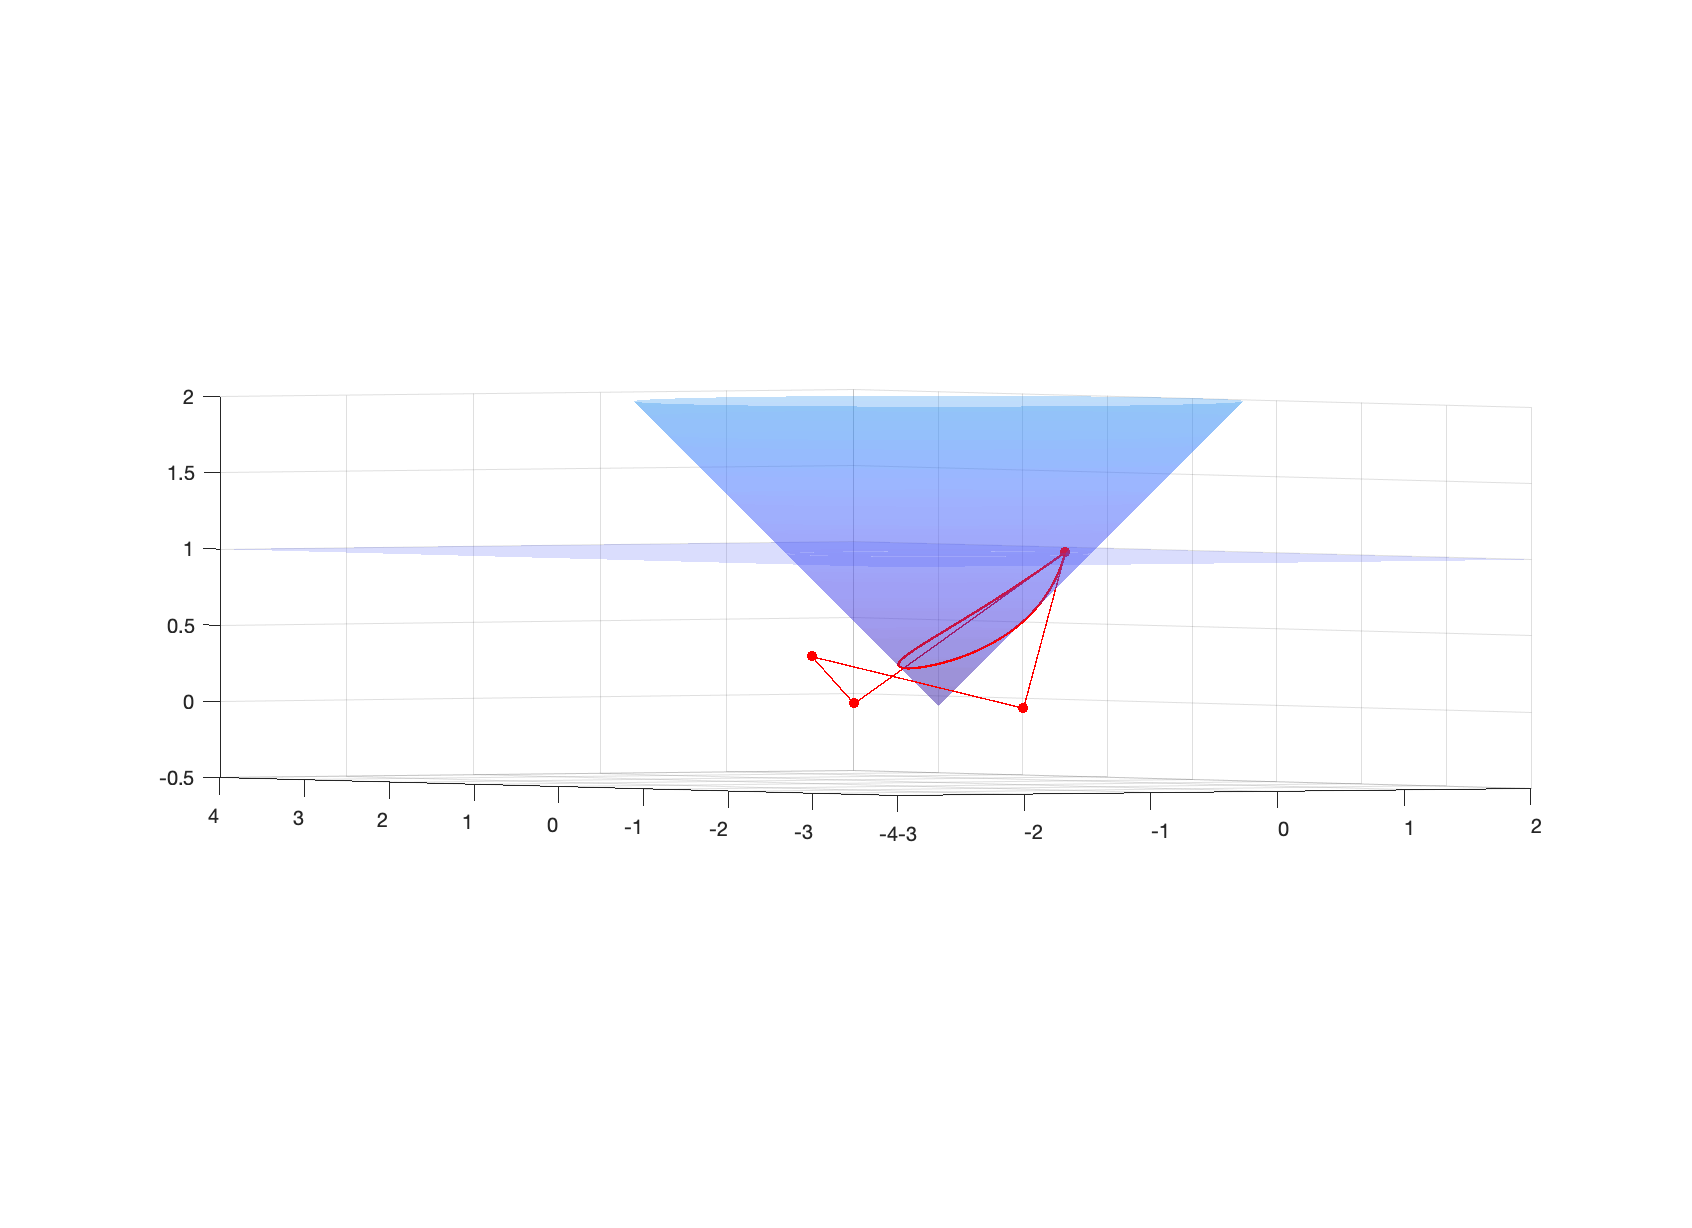
\includegraphics[width=80mm]{kriv4_1b.png}
    \end{minipage}\hfill
    \begin{minipage}{0.5\textwidth}
        \centering
        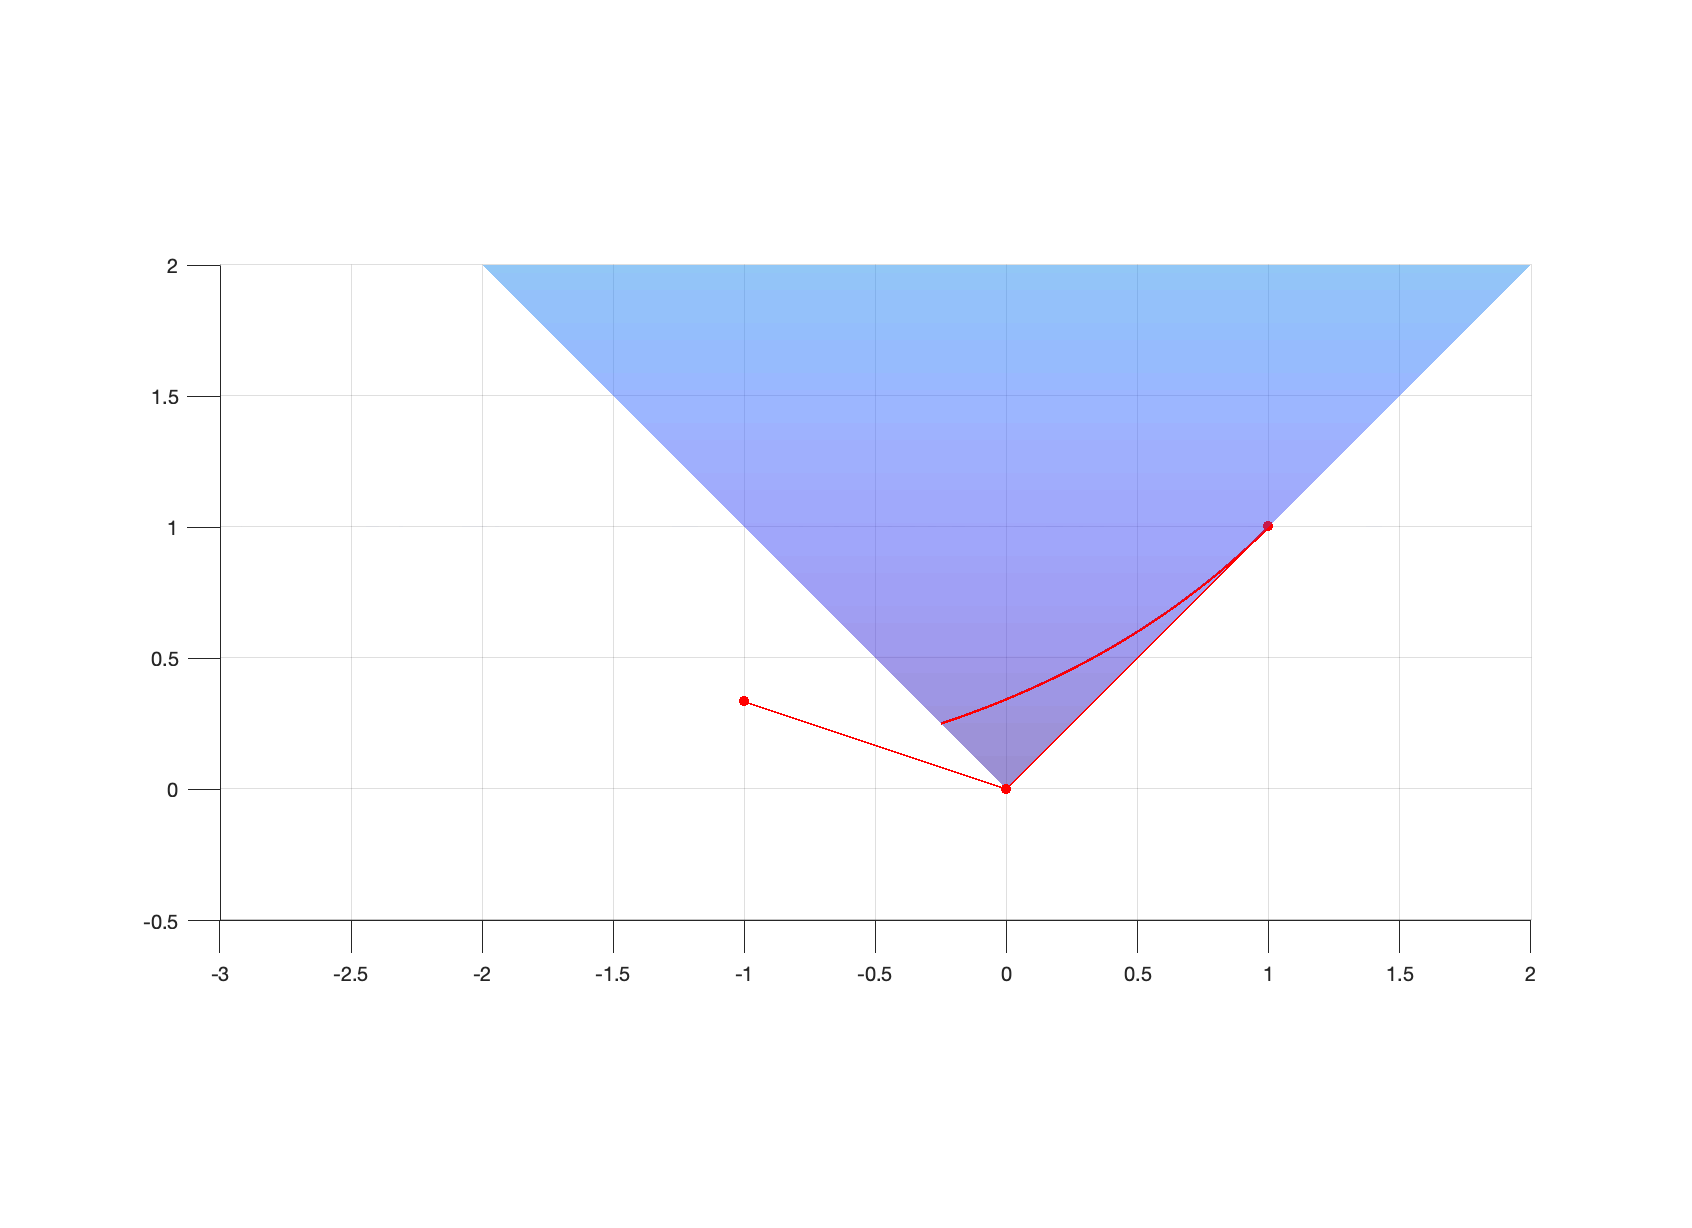
\includegraphics[width=70mm]{kriv4_1c.png}
    \end{minipage}\hfill
    \caption{Primer krivulje 4. stopnje z dvema utežema enakima 0.}
    \label{slika:kriv4}
\end{figure}
\begin{figure}[ht!]
    \begin{minipage}{0.5\textwidth}
        \centering
        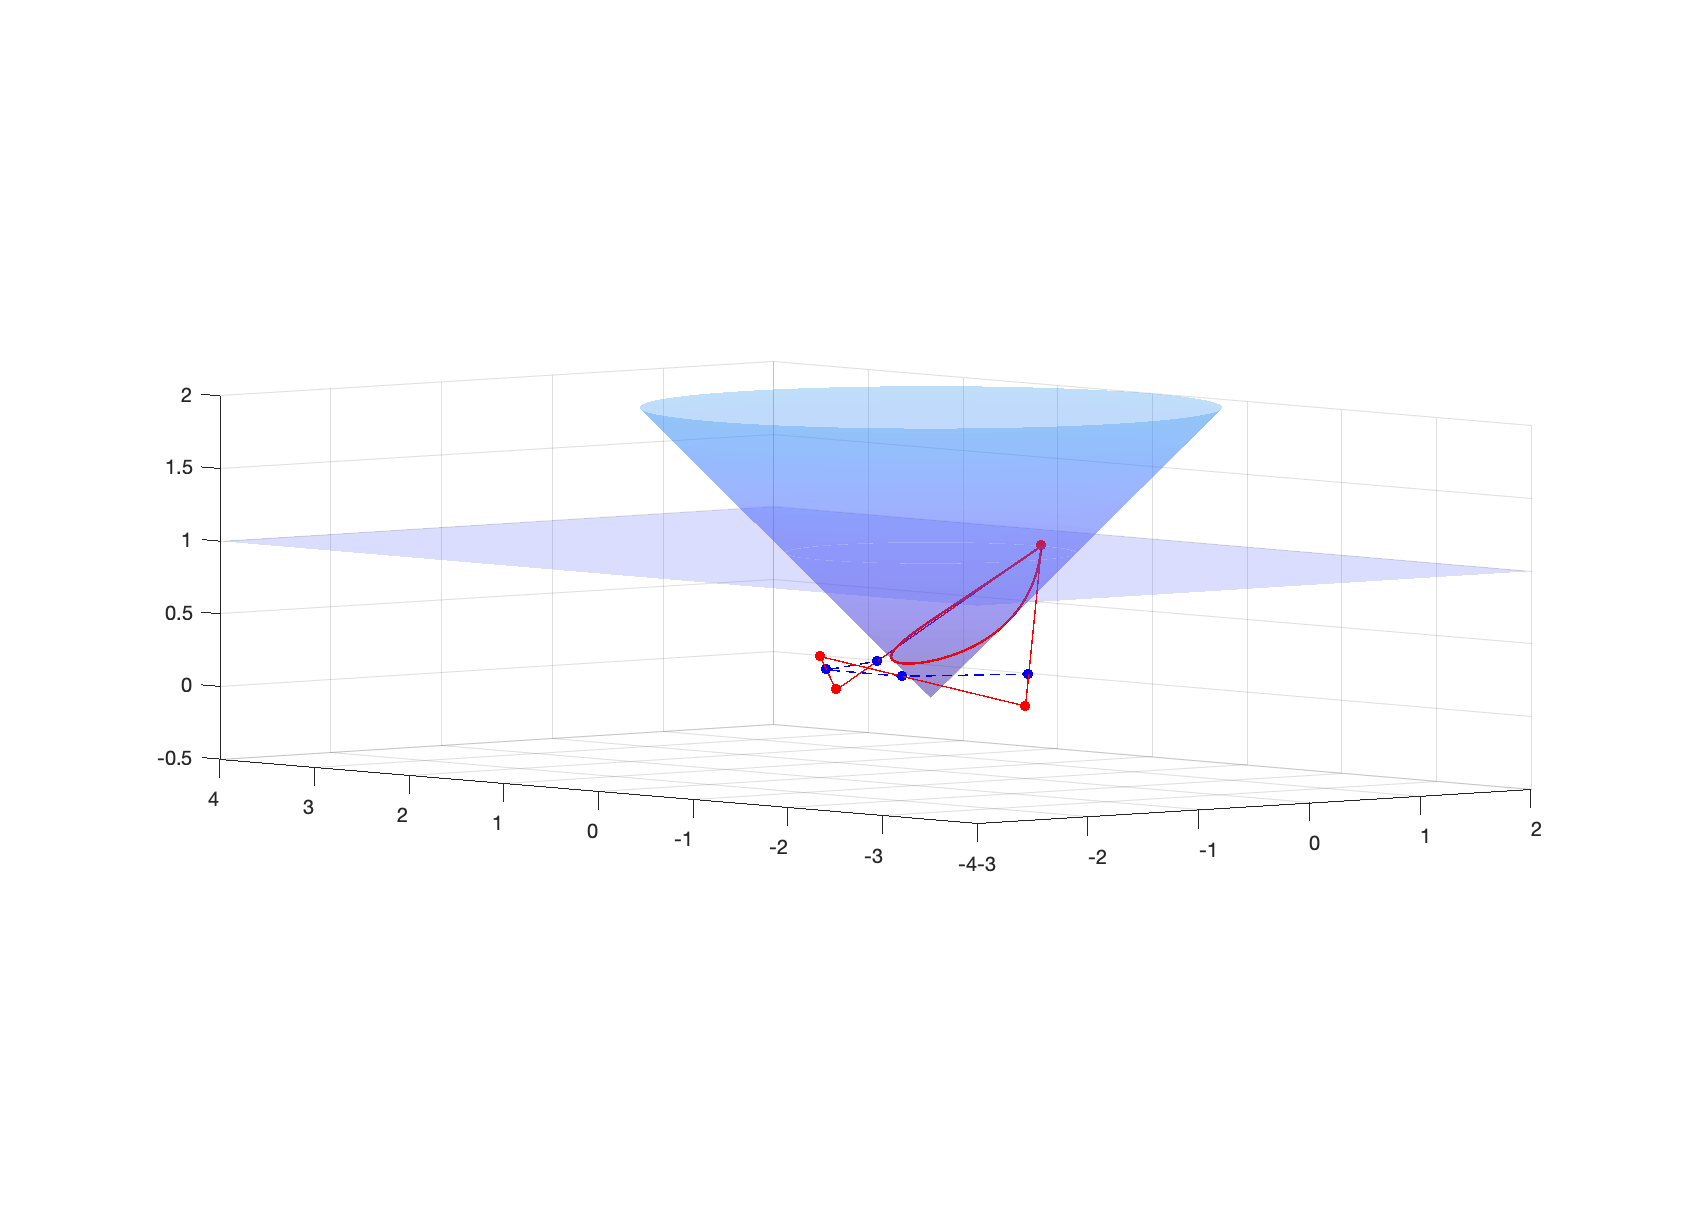
\includegraphics[width=80mm]{kriv4_2a.png}
    \end{minipage}\hfill
    \begin{minipage}{0.5\textwidth}
        \centering
        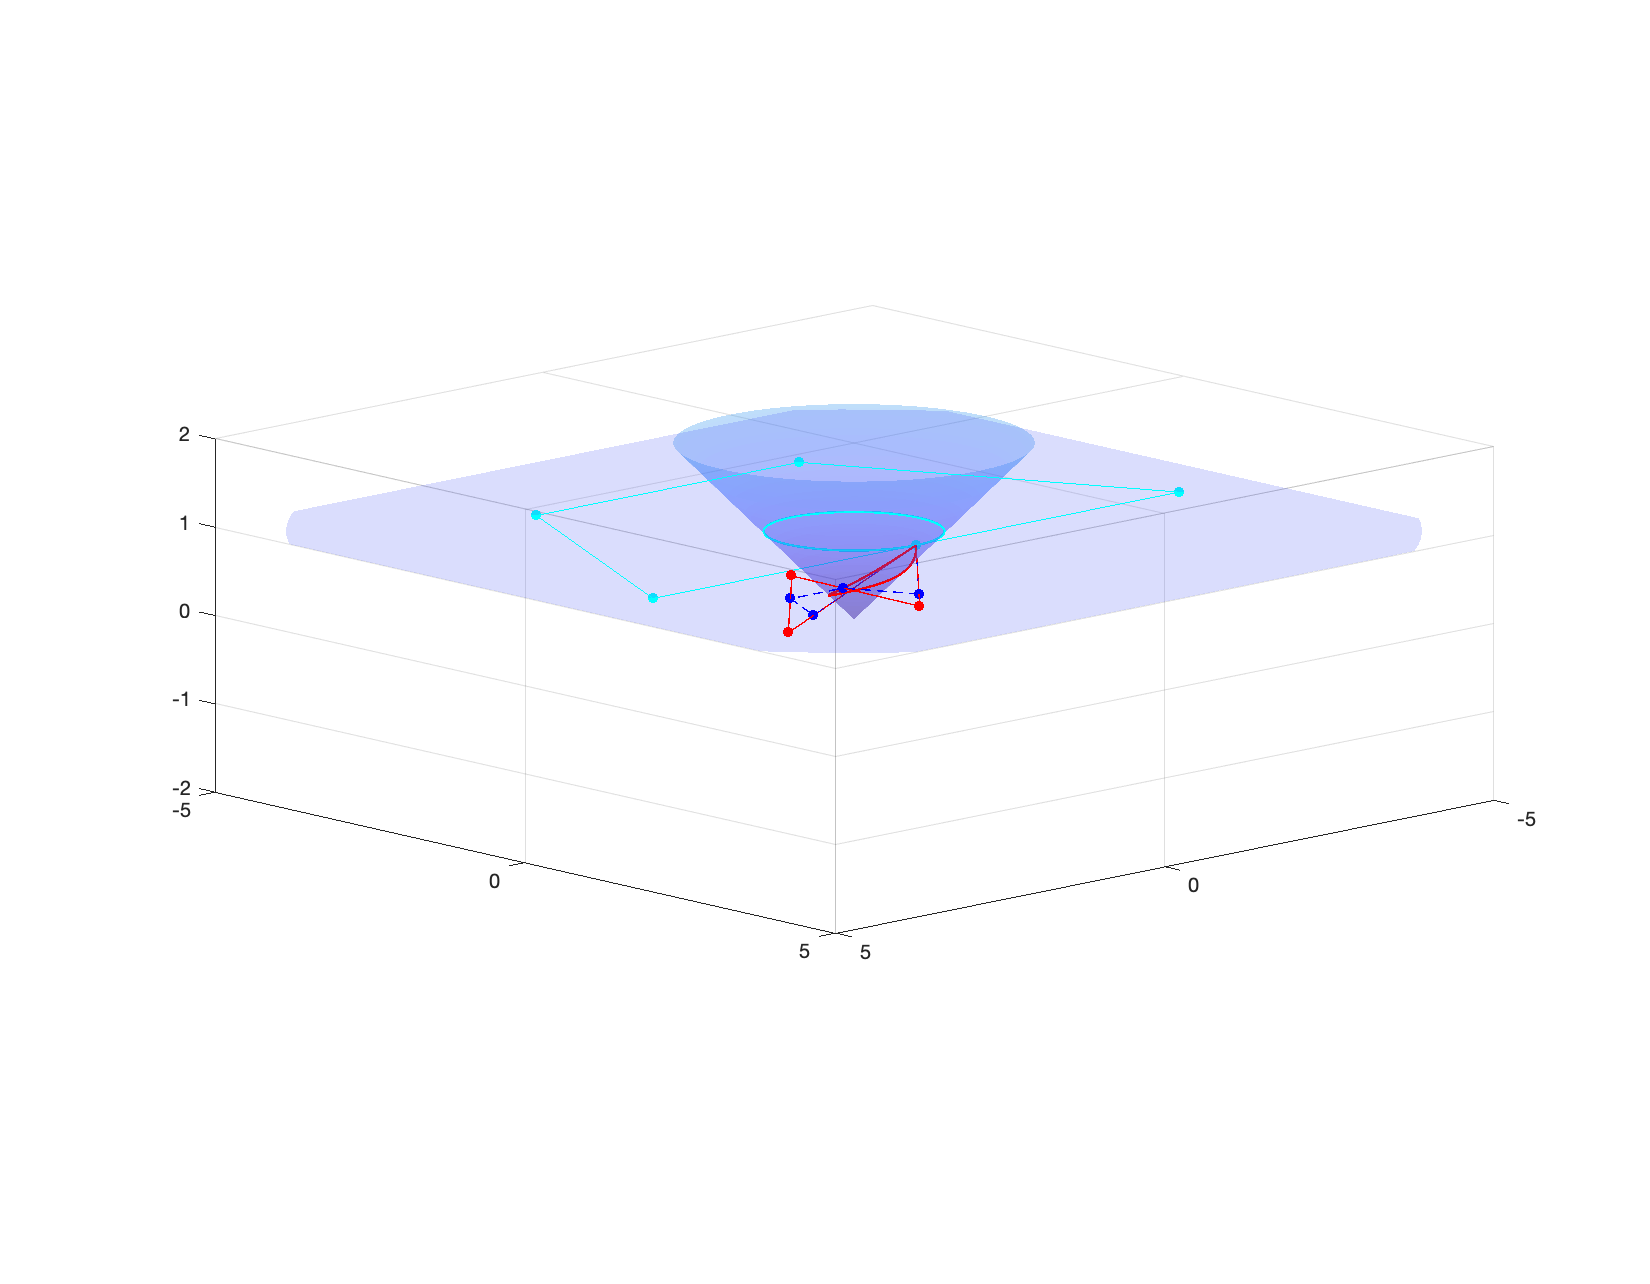
\includegraphics[width=70mm]{kriv4_2c.png}
    \end{minipage}\hfill
    \caption{Primer iste krivulje stopnje 4. kot na sliki \ref{slika:kriv4}, le da je njena stopnja dvignjena. Krivulja ima vse uteži pozitivne. S temno modro barvo je označen poligon krivulje z dvignjeno stopnjo.}
    \label{slika:kriv4a}
\end{figure}
\begin{figure}[ht!]
    \begin{minipage}{0.5\textwidth}
        \centering
        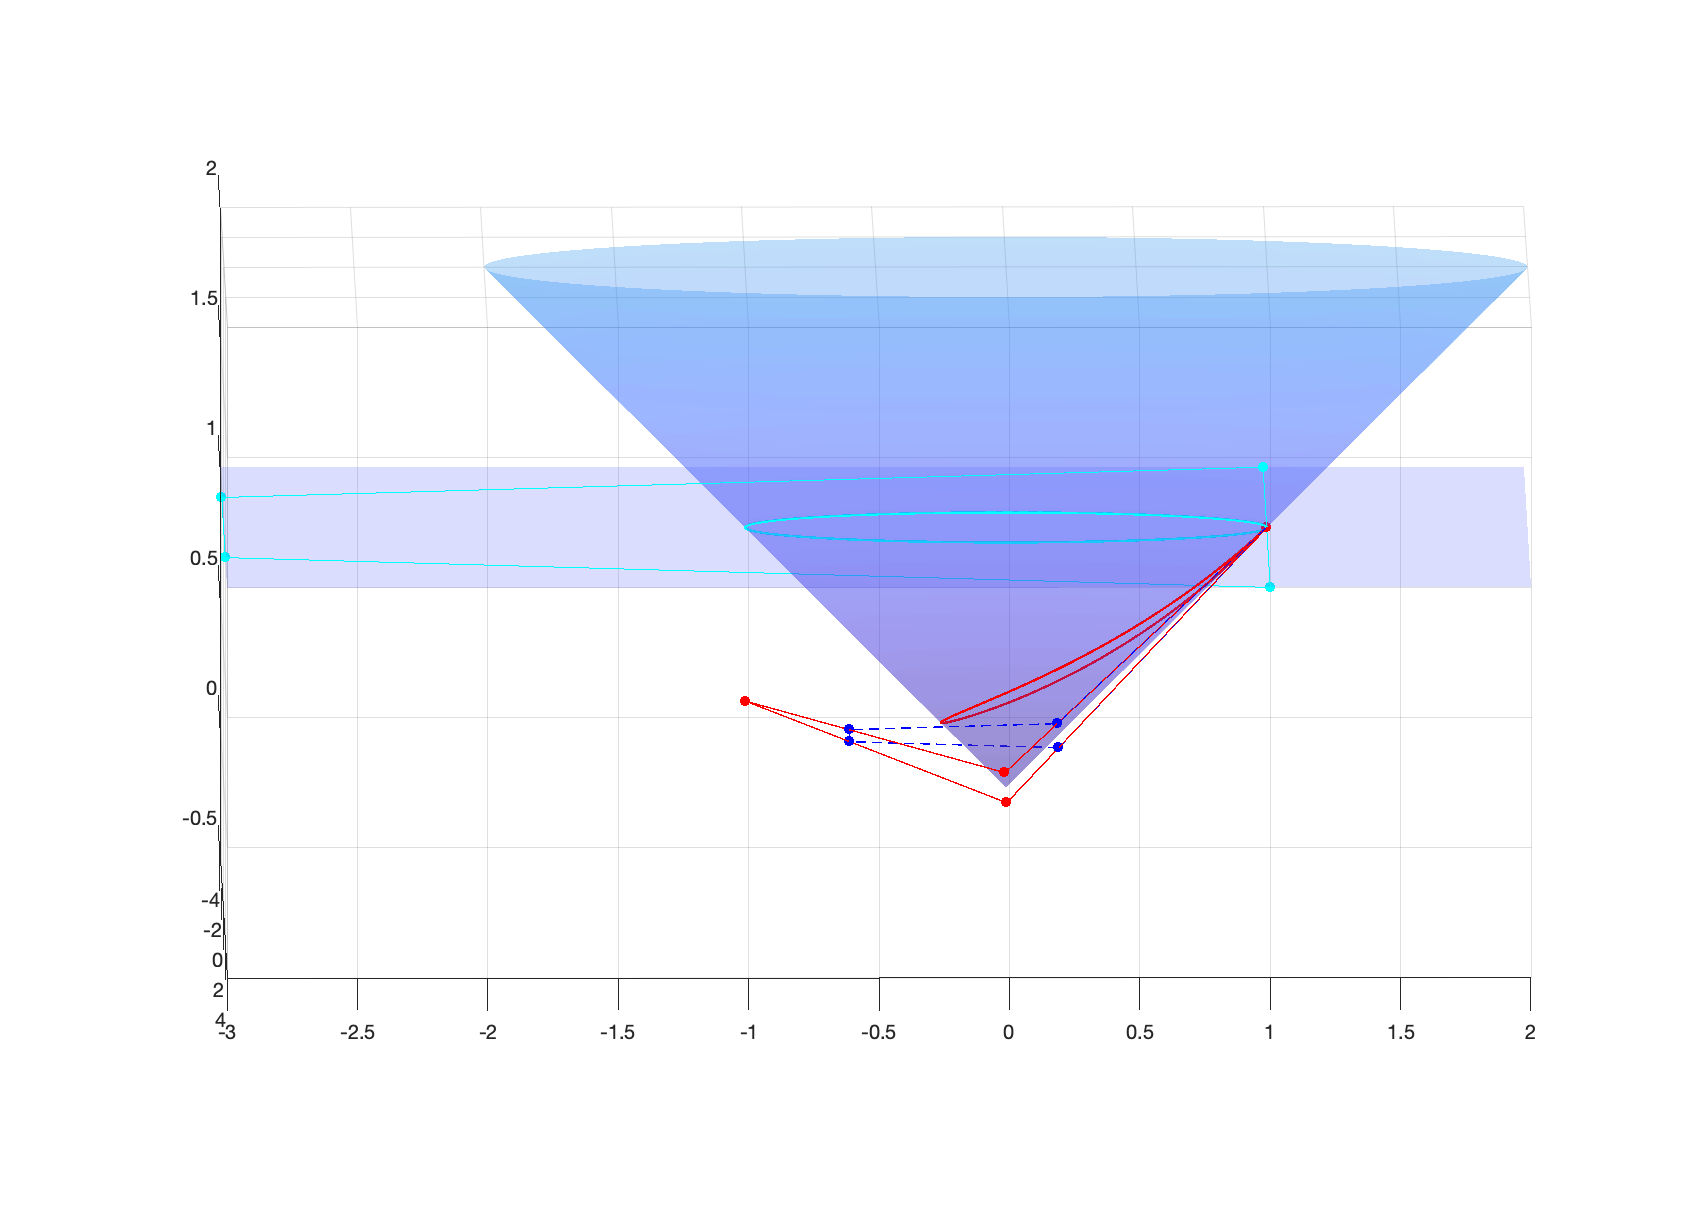
\includegraphics[width=80mm]{kriv4_3a.png}
    \end{minipage}\hfill
    \begin{minipage}{0.5\textwidth}
        \centering
        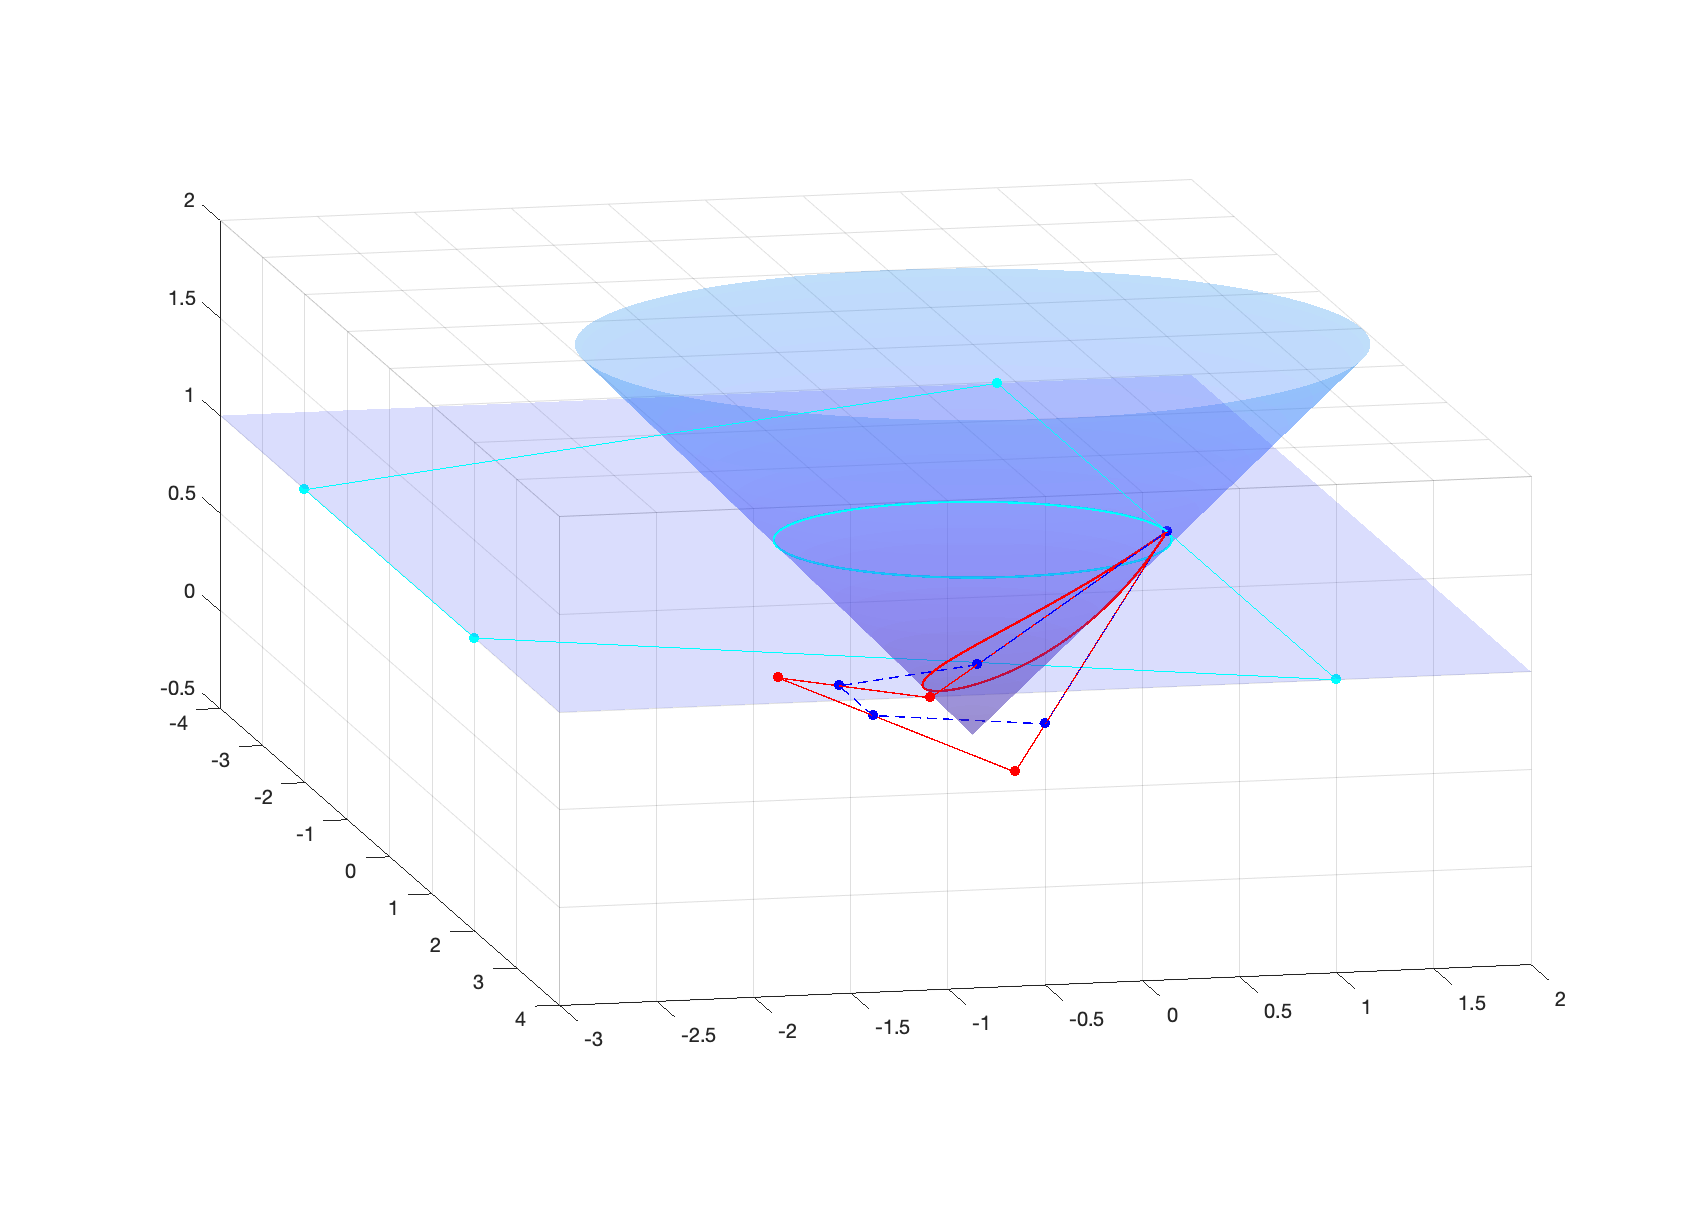
\includegraphics[width=80mm]{kriv4_3b.png}
    \end{minipage}\hfill
    \caption{Primer iste krivulje stopnje 4. kot na slikah \ref{slika:kriv4} in \ref{slika:kriv4a}. S svetlo modro barvo sta označena projecirana krivulja na ravnino $w = 1$ in njen kontrolni poligon.}
\end{figure}


%%%%%%%%%%%%%%%%%%%%%%%%%%%%%%%%%%%%%%%%%%%%%%%%%%%%%%%%%%%%%%%%%%%%%%%%%%%%%%%%%%%%%%

\section{Kubični B\'ezierjev krožni lok}


Zanima nas, kakšne krožne loke lahko opišemo s kubično racionalno B\'ezierjevo krivuljo pri pogoju, da so vse uteži nenegativne. Da dobimo pogoje za kontrolne točke B\'ezierjeve krivulje, krivuljo vstavimo v enačbo stožca
$$ \tilde{X}(t)^2+\tilde{Y}(t)^2-W(t)^2=0.$$
\begin{align*}
\tilde{X}(t) &= \tilde{x}_0\cdot B_0^3(t)+\tilde{x}_1\cdot B_1^3(t)+ \tilde{x}_2\cdot B_2^3(t) + \tilde{x}_3\cdot B_3^3(t) = \\
&= \tilde{x}_0\cdot (1-t)^3+\tilde{x}_1\cdot3t(1-t)^2+\tilde{x}_2\cdot3t^2(1-t)+\tilde{x}_3\cdot t^3 \\
\tilde{Y}(t) &=\tilde{y}_0\cdot B_0^3(t)+\tilde{y}_1\cdot B_1^3(t)+\tilde{y}_2\cdot B_2^3(t) + \tilde{y}_3\cdot B_3^3(t) = \\
&= \tilde{y}_0\cdot (1-t)^3+\tilde{y}_1\cdot3t(1-t)^2+\tilde{y}_2\cdot3t^2(1-t)+\tilde{y}_3\cdot t^3 
\end{align*}
$\tilde{X}(t)$ in $\tilde{Y}(t)$ kvadriramo, zato moramo množiti Bernsteinove bazne polinome:
$$B_i^n(t)\cdot B_j^m(t)=\frac{\binom{n}{i} \cdot \binom{m}{j}}{\binom{n+m}{i+j}}B_{i+j}^{n+m}(t).$$
Iz tega dobimo sedem enačb.\\
Spomnimo se, da smo pri kvadratični krivulji izbrali za prvo in zadnjo točko dve točki, ki ležita na krožnici, srednjo točko pa na polovičnem kotu med njima. Tudi tu lahko predpostavimo, da sta prva in zadnja točka na krožnici:
\begin{align*}
\boldsymbol{\tilde{b}}_0 &= (\cos \theta, -\sin \theta, 1)\\
\boldsymbol{\tilde{b}}_3 &= (\cos \theta, \sin \theta, 1),
\end{align*}
kjer je $\theta$ polovični kot krožnega loka.  S tem se nam sedem enačb poenostavi v pet enačb:
\begin{align*}
w_1 = \tilde{x_1}\cos{\theta} - \tilde{y_1} \sin{\theta}   \\
w_2 = \tilde{x_2}\cos{\theta} + \tilde{y_2} \sin{\theta}   \\
3\tilde{x_1}^2\sin^2{\theta} + 3\tilde{y_1}^2\cos^2{\theta} - 4\tilde{y_2} \sin{\theta}  + 6\tilde{x_1}\tilde{y_1} \sin{\theta} \cos{\theta} = 0 \\
9\tilde{x_1}\tilde{x_2}\sin^2{\theta} + 9\tilde{y_1}\tilde{x_2}\cos{\theta} \sin{\theta} - 9\tilde{x_1} \tilde{y_2} \cos{\theta} \sin{\theta}+ \\
+ 9 (1 + \sin^2{\theta}) \tilde{y_1} \tilde{y_2} - 2\sin^2{\theta} = 0 \\
3\tilde{x_2}^2 \sin^2{\theta}+ 3\tilde{y_2}^2 \cos^2{\theta}+ 4\tilde{y_1} \sin{\theta}  - 6\tilde{x_2}\tilde{y_2}\sin{\theta} \cos{\theta}  = 0 
\end{align*}

\begin{zgled}
Poglejmo si, kaj je rešitev sistema, če vzamemo $\theta= \frac{\pi}{2}$. Dobimo naslednje kontrolne točke:

\begin{align*}
\boldsymbol{\tilde{b}}_0 &= (0,-1,1) \\
\boldsymbol{\tilde{b}}_1 &= (\frac{2\alpha}{3},-\frac{1}{3\alpha^2},\frac{1}{3\alpha^2}) \\
\boldsymbol{\tilde{b}}_2 &= (\frac{2}{3\alpha},\frac{\alpha^2}{3},\frac{\alpha^2}{3}) \\
\boldsymbol{\tilde{b}}_3 &= (0,1,1)
\end{align*}
kjer je $\alpha=\frac{3\tilde{x_1}}{2}$. \\
Kontrolne točke v 2D so $\boldsymbol{b}_0 = (0,-1),\boldsymbol{b}_1 = (2\alpha^3,-1),\boldsymbol{b}_2 = (\frac{2}{\alpha^3},1),\boldsymbol{b}_3 = (0,1)$.
\end{zgled}

Ker je kot $\theta$ spremenljivka, je iz zgornjega sistema enačb težko dobiti eksplicitno rešitev. Zato si bomo v nadaljevanju ogledali drugačen pristop za iskanje kubičnih B\'ezierjevih krožnih lokov, pomagali si bomo s spodnjim izrekom.

\begin{izrek}
Če je krivulja
$$\boldsymbol{C}(t)=\frac{(\tilde{X}(t),\tilde{Y}(t))}{W(t)}$$
omejena za $t\in [-\infty,\infty]$ in so $\tilde{X}(t),\tilde{Y}(t)$ in $W(t)$ polinomi brez skupnih deliteljev, potem noben izmed $\tilde{X}(t),\tilde{Y}(t)$ in $W(t)$ ni lihe stopnje.
\end{izrek}

\begin{proof}
Najdemo ga v \cite{chou}.
\end{proof}

\noindent
Iz izreka sledi, da so edini možni kubični B\'ezierjevi krožni loki oblike
$$\boldsymbol{C}(t)=\frac{(\tilde{X}(t),\tilde{Y}(t))(aB_0^1(t)+bB_1^1(t))}{W(t)(aB_0^1(t)+bB_1^1(t))},$$
kjer je $$\frac{(\tilde{X}(t),\tilde{Y}(t))}{W(t)}$$
kvadratični krožni lok.\\

\noindent
Za kontrolni poligon kvadratičnega krožnega loka izberemo
\begin{align*}
\boldsymbol{\tilde{b}}_0 &= (\cos{\theta}, -\sin{\theta}, 1)\\
\boldsymbol{\tilde{b}}_1 &= (\sqrt{w_2}, 0,\sqrt{w_2} \cos{\theta})\\
\boldsymbol{\tilde{b}}_2 &= (w_2\cos \theta, w_2 \sin\theta, w_2),
\end{align*}
kjer je $\theta$ polovični kot krožnega loka. Tu so kontrolne točke izbrane podobno kot v \ref{kvadraticna}, kjer je sedaj $w_2$ prosta utež.

Imenovalec kubične krivulje je enak
\begin{align*}
W(t)(aB_0^1(t)+bB_1^1(t)) &= aB_0^3(t)+\left ( \frac{2}{3}a\sqrt{w_2}\cos \theta +\frac{b}{3} \right )B_1^3(t)+ \\
&+ \left ( \frac{aw_2}{3} + \frac{2}{3}b\sqrt{w_2}\cos \theta  \right )B_2^3(t) + bw_2B_3^3(t)
\end{align*}

Za $w_0'$ in $w_3'$ mora veljati
\begin{align*}
w_0'&=a \\
w_3'&=bw_2
\end{align*}
Brez škode za splošnost lahko uteži postavimo v standardno obliko, tedaj sta $w_0'$ in $w_3'$ enaki $1$. Iz tega sledi
$$ a=1 \quad \text{ in } \quad w_2=\frac{1}{b}.$$
Iz tega sledi, da so kontrolne točke kubičnega B\'ezierjevega krožnega loka enake
\begin{align*}
\boldsymbol{\tilde{b}}_0 &= (\cos{\theta}, -\sin{\theta}, 1)\\
\boldsymbol{\tilde{b}}_1 &= \left ( \left (\frac{2}{3\sqrt{b}}+\frac{b\cos \theta}{3}\right ),-\frac{b \sin \theta}{3},\left (\frac{2\cos \theta}{3\sqrt{b}}+\frac{b}{3}\right )\right )\\
\boldsymbol{\tilde{b}}_2 &= \left ( \left (\frac{\cos \theta}{3b}+\frac{2\sqrt{b}}{3}\right ),\frac{\sin \theta}{3b},\left (\frac{2\sqrt{b}\cos \theta}{3}+\frac{1}{3b}\right )\right )\\
\boldsymbol{\tilde{b}}_3 &= (\cos \theta, \sin\theta, 1),
\end{align*}
Ker želimo imeti nenegativne uteži, mora veljati še
$$\frac{2\cos \theta}{3\sqrt{b}}+\frac{b}{3}\geq0$$
in
$$\frac{2\sqrt{b}\cos \theta}{3}+\frac{1}{3b}\geq0.$$
Iz tega sledi
$$\cos \theta \geq -\frac{b^{3/2}}{2}\quad\text{ in }\quad \cos  \theta \geq -\frac{1}{2b^{3/2}}.$$
Označimo $\beta=b^{3/2}$ in si oglejmo funkciji $y=-\frac{\beta}{2}$ in $y=-\frac{1}{2\beta}$.\\
\begin{figure}[ht!]
    \centering
    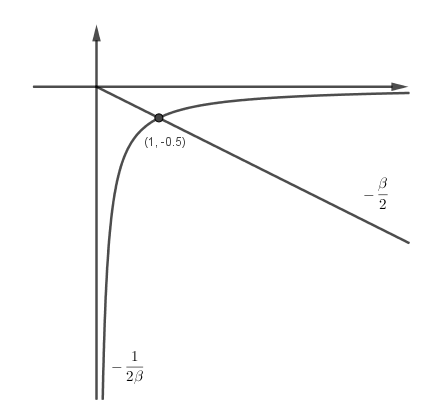
\includegraphics[width=80mm]{graf.png}
    \caption{Grafa funkcij $y=-\frac{\beta}{2}$ in $y=-\frac{1}{2\beta}$ Slika je povzeta po \cite{chou}.}
    \label{slika:graf}
\end{figure}
\\
Maksimalen kot $\theta$ dosežemo pri $b=1$, in sicer $\theta=120^{\circ}$. Ker je $\theta$ polovični kot krožnega loka, je maksimalen krožni lok, ki ga lahko opišemo s kubično B\'ezierjevo krivuljo z nenegativnimi utežmi enak $240^{\circ}$.
%%%%%%%%%%%%%%%%%%%%%%%%%%%%%%%%%%%%%%%%%%%%%%%%%%%%%%%%%%%%%%%%%%%%%%%%%%%%%%%%%%%%%%
\newpage
\begin{thebibliography}{99}
\bibitem{chou}
J.~J.~Chou, \emph{Higher order Bezier circles}, Computer-Aided Design \textbf{27 (4)} (1995) 303--309

\bibitem{farin}
G.~Farin, \emph{Curves and surfaces for CAGD}, A Practical Guide, 5th ed., Morgan Kaufmann, 2002, poglavje 12.7

\bibitem{knez}
M.~Knez, J.~Grošelj, \emph{Računalniško podprto geometrijsko oblikovanje}, ... (2020)
\end{thebibliography}


\end{document}